\section{Analysis}
\subsection{The Impact of Selected Feature Numbers}
A unique hyperparameter in~\modelname~could be $K$ for the selection of last features which determines how many highest scores to be included to form the final feature vectors.
To explore how $K$ affects the model's performance, we run our model with various values of $K$ and plot how the performance changes in Figure~\ref{fig:perf_kvalue}.
It can be found that to achieve ideal performance in both datasets, an appropriate choice of $K$ (from 64 to 128) is necessary. 
When setting $K$ too high or too low, i.e., dispersing the model's concentration on too many scores or forcing the model to focus on only a few highest scores, the model fails to reach the optimum. 
This phenomenon reveals that a promising filter should provide comprehensive coverage of the matching scores for the prediction layer.

\begin{figure}[ht!]
    \centering
    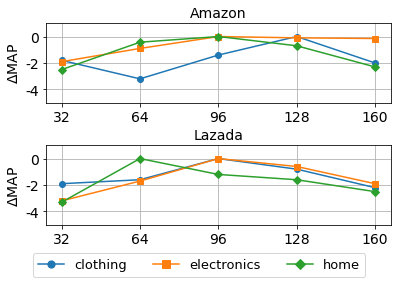
\includegraphics[scale=0.5]{Contents/img/ablative.png}
    \caption{The relative MAP drop (the absolute value of $\Delta$MAP) from the optim to different $K$.
    Performance when $K>160$ or $K<32$ is far lower than the optimum so we do not include in the figure.}
    \label{fig:perf_kvalue}
\end{figure}

\subsection{The Impact of Lower Layer Filter}
Apart from the last-layer feature selector, we also insert many filters into the lower layers. 
To verify the efficacy of this design, we performed additional experiments by varying $r_{min}$~in~\cref{alg:1} while fixing $K=96$ and $C=\lceil\sqrt{K}\rceil=10$. 
The results on the two datasets are shown in~\Cref{fig:perf_cluster}, from which we notice that in all categories, a proper choice of $r$ value ($k=4$ in our experiments) can further enhance the performance by removing duplicated semantics in lower aggregation layers. 
This suggests that the semantics redundancy removal procedure the combination of $k$-means and random sampling can serve as a primary filter for the feature selection.

\begin{figure}
    \centering
    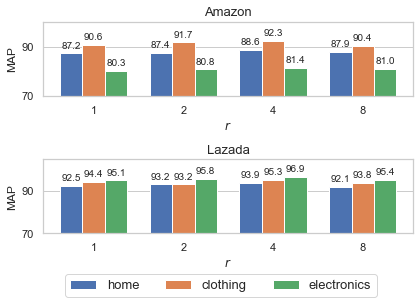
\includegraphics[scale=0.5]{Contents/img/cluster.png}
    \caption{The performance (MAP) under different $r$ on two datasets.}
    \label{fig:perf_cluster}
\end{figure}

\subsection{Why Does BERT Fail?}
\label{sec:bert_fail}
As mentioned above, it is weird that after replacing the word vectors (GloVe and FastText) with the pretrained language model in the embedding layer, both the fusion-based and fusion-free models fail to produce a significant increase as in other multimodal tasks. 
We surmise that this is mainly due to informal text input.
Upon manual inspection, we find many pieces of low-quality reviews---especially those of low helpfulness scores.
Take review 2 in Table~\ref{Problem Setting} as an example, 
the review passage is readable by sentence except for some grammatical errors, but the logic is messy and out of the topic. 
The results of previous work on tasks related to spoken language (informal text) have shown that BERT may not lead to a performance improvement~\citep{gu2020data}.
% In~\cref{sec:bert_fail}, we qualitatively give some explanation about the seemingly abnormal BERT results.
To further verify our hypothesis, we carry out a group of blank control experiments on Amazon-MRHP dataset.
Specifically, we run regression directly on: A) representations encoded by a single layer GRU with Glove 300d as word embeddings in both fields; B) the representations at the position of [CLS] token using BERT-base-uncased as the pretrained encoder. 
The results are shown in Table~\ref{tab:bert_studyl}.
From the table we find the performance between word vectors and BERT pretrained models are very close. 
This outcome looks consistent with the results in~\citet{gu2020data} and may substantiate our aforementioned hypothesis.

\begin{table}[h]
    \centering
    \begin{tabular}{c|c|c|c|c}
        \toprule
        Category & Setting & MAP & N@3 & N@5 \\
        \midrule
        \multirow{2}{*}{Clothing} & A & 64.83 & 55.62 & 58.95   \\
         ~ & B & 64.75 & 55.51 & 59.03   \\
        \midrule 
        \multirow{2}{*}{Electronics} & A & 53.63 & 43.77 & 47.31  \\
         ~ & B & 53.90 & 43.85 & 47.02 \\
         \midrule
        \multirow{2}{*}{Home} & A & 61.08 & 51.17 & 54.26 \\
         ~ & B & 61.03 & 51.09 & 54.14 \\
         \bottomrule
    \end{tabular}
    \caption{A group of blank control experiments on Amazon-MRHP dataset.}
    \label{tab:bert_studyl}
\end{table}




